% !TEX program = xeLaTeX

\documentclass[12pt, a4paper, twoside]{article}
\usepackage[margin=1in]{geometry}
% support for CJK
\usepackage{xeCJK}
% support for graphics
\usepackage{graphicx}
% support for colors
\usepackage{xcolor}
\definecolor{dkgreen}{rgb}{0,0.6,0}
\definecolor{gray}{rgb}{0.5,0.5,0.5}
\definecolor{mauve}{rgb}{0.58,0,0.82}
% math packages
\usepackage{amsmath, amsthm, amssymb, bm}
% hyper references
\usepackage{hyperref}
\hypersetup{colorlinks=true, urlcolor=blue, linkcolor=blue, citecolor=blue}
% scientific units
\usepackage[separate-uncertainty = true]{siunitx}
\DeclareSIUnit\pixel{px}
% typesetting chemistry
\usepackage{mhchem}
% citations and references
% \usepackage[style=apa, backend=biber, sorting=nyt]{biblatex}
% additional symbols
\usepackage{gensymb}
\usepackage{textcomp}
% indent first paragraphs
\usepackage{indentfirst}
% ordinal numbers
\usepackage[super]{nth}
% more formatting for tables
\usepackage{multirow, makecell}
% typesetting program codes
\usepackage{listings}
\lstdefinestyle{python}{frame=tb,
  language=Python,
  aboveskip=3mm,
  belowskip=3mm,
  showstringspaces=false,
  columns=flexible,
  basicstyle={\small\ttfamily},
  numbers=left,
  numberstyle=\tiny\color{gray},
  keywordstyle=\color{blue},
  commentstyle=\color{dkgreen},
  stringstyle=\color{mauve},
  breaklines=true,
  breakatwhitespace=true,
  escapeinside=``,
  tabsize=4,
  extendedchars=false
}
\lstdefinestyle{output}{
  language=,
  basicstyle=\ttfamily,
  columns=fullflexible,
  breaklines=true,
  keepspaces=true,
  showstringspaces=false,
  frame=single,
  xleftmargin=5pt,
  xrightmargin=5pt,
}
\lstset{style=python}
\usepackage{tikz}
\usetikzlibrary{arrows.meta}
\usepackage{subcaption}

\title{\texttt{obfusimg} 简要文档}
\author{\_\_roselle\_\_, pigeon.hannah}

\makeatletter
\let\thetitle\@title
\let\theauthor\@author
\makeatother
\usepackage{fancyhdr}
\fancyhead[RO,LE]{\theauthor}
\fancyhead[LO,RE]{\thetitle}
\pagestyle{fancy}

% \addbibresource{citations.bib}

\begin{document}

\maketitle

\begin{abstract}
    \texttt{obfusimg} 应用提供了多种算法，用于以确定且可逆的方式打乱图像像素，从而实现图像混淆。本文档作为该应用 C++ 实现的一份半技术型使用说明。
\end{abstract}

\section{引言} \label{intro}

可逆图像混淆有着广泛的应用场景，从保护隐私的图像分享（例如绕过审查）到科学与工业图像流程中的可逆预处理（例如在空间相关性被打乱的条件下对机器学习架构进行基准测试）。

一种相对直接的混淆方法是重新排列给定图像中的全部像素。每个像素按照某种规则被移动到一个唯一的新位置，使得输出图像具有相同的尺寸（宽度、高度、通道数），但几乎无法辨认（见图~\ref{fig:rearranging_pixels_is_effective}）。

\begin{figure}[b!]
    \centering
    \begin{subfigure}[t]{0.5\textwidth}
        \centering
        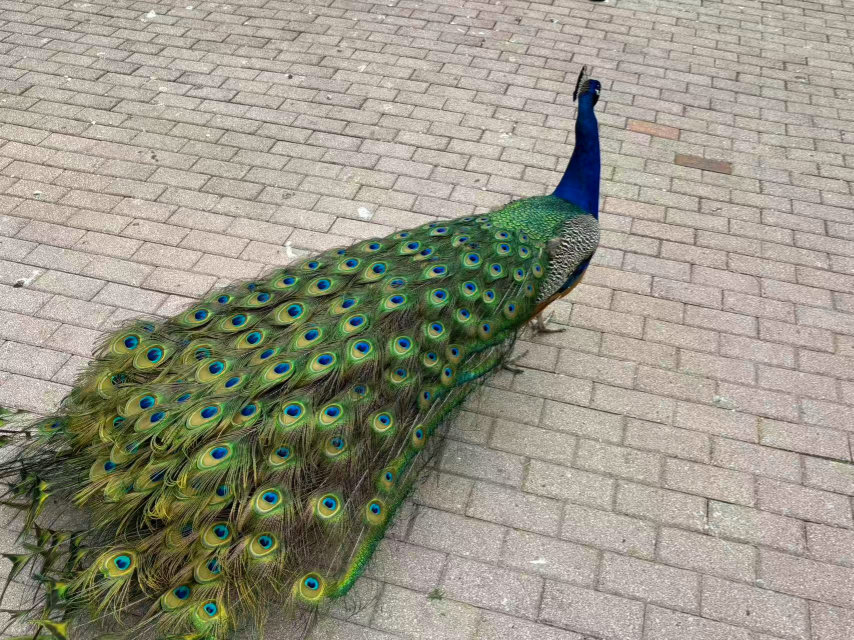
\includegraphics[width=.7\textwidth]{figures/demo_peacock.jpg}
        \caption{一张孔雀图像（由 mnrva 提供）。}
    \end{subfigure}%
    ~
    \begin{subfigure}[t]{0.5\textwidth}
        \centering
        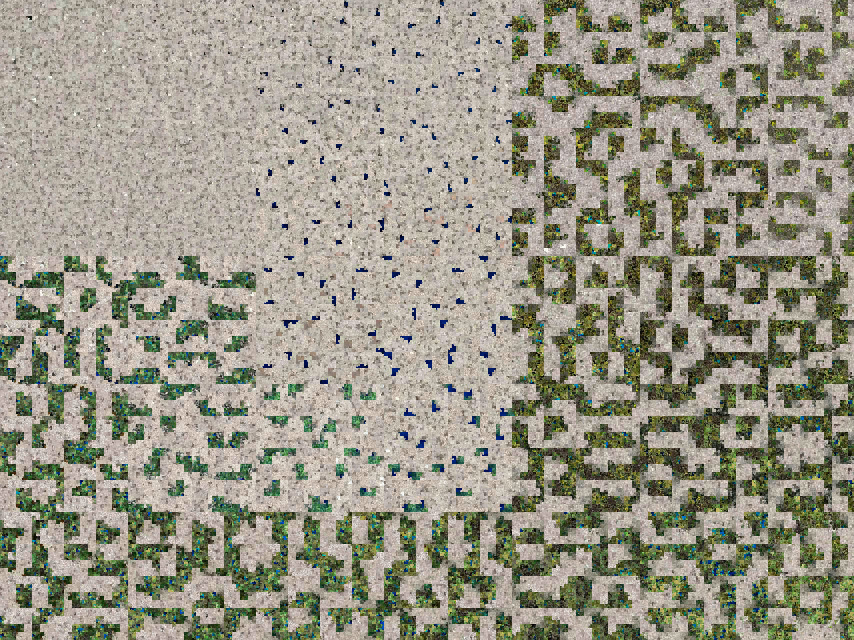
\includegraphics[width=.7\textwidth]{figures/demo_peacock_out.jpg}
        \caption{所有像素被重排后的孔雀图像。}
    \end{subfigure}
    \caption{示例图像中的孔雀在所有像素被重排后变得无法辨认。当前最先进的 LLM 也无法稳定识别该混淆图像的主体（在 ChatGPT 5.2 Thinking extended 上测试）。}
    \label{fig:rearranging_pixels_is_effective}    
\end{figure}

应用 \texttt{obfusimg} 实现了多种生成此类像素重排的方法。尤其是，这些算法的计算成本较低，用户可以在任何合理的本地设备上运行该应用，这意味着在混淆之前无需通过互联网传输任何信息。

\section{图像与混淆的数学模型}

设一幅图像的宽为 $w$ \si{\pixel}、高为 $h$ \si{\pixel}，并具有 $c$ 个通道（通常 \texttt{jpeg} 文件的 RGB 图像有 $c = 3$，\texttt{png} 文件的 RGB+Alpha 图像有 $c = 4$）。我们将图像识别为一个 $1$ 维数组
\begin{equation}
    A = \bigl(a_0, a_1 \ldots, a_{w h - 1}\bigr)
\end{equation}
其中每个 $a_i$ 存储一个像素的全部 $c$ 个通道值（通常每个通道值是整数 $0 \leq n \leq 255$）。这里我们采用行优先（row-major）索引：若原图中某像素坐标为 $(x, y)$，且
\begin{equation}
    0 \leq x < w, \qquad 0 \leq y < h,
\end{equation}
则其数组下标为
\begin{equation}
    i = i(x, y) = y w + x.
\end{equation}
这意味着我们按从左到右、从上到下的顺序读取像素。只要知道图像的宽（或高），这个过程就是可逆的。

于是，通过重排全部像素得到的一种混淆方法可定义为一个置换\footnote{映射 $f\colon A \to A$ 若是双射，则称为 $A$ 上的一个置换。因此，置换 $f\colon A \to A$ 必然存在唯一逆映射 $f^{-1}\colon A \to A$。}
\begin{equation}
    \sigma\colon \{0, 1, \ldots, w h - 1 \} \to \{0, 1, \ldots, w h - 1 \}
\end{equation}
并且混淆后的图像为
\begin{equation}
    A' = \bigl(a_{\sigma(n)}\bigr)_n.
\end{equation}
换言之，混淆图像中的第 $n$ 个像素对应于原图中的第 $\sigma(n)$ 个像素。对 $A'$ 应用逆混淆方法 $\sigma^{-1}$ 可得
\begin{equation}
    A'' = \bigl(a_{\sigma^{-1}(\sigma(n))}\bigr)_n = \bigl(a_{n}\bigr)_n = A
\end{equation}
从而恢复原图。

\section{混淆算法}

在 \texttt{obfusimg} 中实现的每种算法本质上都是一个映射
\begin{equation}
    \alpha\colon \mathcal{I} \times [0, 1) \to \mathcal{P}, (I, s) \to \sigma
\end{equation}
其中 $\mathcal{I}$ 是所有图像的集合，$\mathcal{P}$ 是所有有限集合置换的集合，$I = (w, h, c, A)$ 是用户输入图像，$s \in [0, 1)$ 是用户定义的种子（seed），而 $\sigma$ 是集合 $\{0, 1, \ldots, w h - 1\}$ 上的一个置换。实际中，$\alpha(I, s)$ 几乎从不依赖于 $c$ 和 $A$，因为 $c$ 的变化很小，而对于 \texttt{jpeg} 文件来说，$A$ 又容易受到有损压缩影响。

\subsection{G/Hilbert 曲线}

对于一个 $2^n \times 2^n$ 的正方形，Hilbert 曲线\footnote{严格来说，我们使用的是趋向 Hilbert 曲线的有限次迭代曲线。Hilbert 曲线与 Peano 曲线一样，都是空间填充曲线，并且是从 $[0,1]$ 到 $[0,1]^2$ 的\emph{连续}双射映射的例子。这一点颇为反直觉，因为低维长方体的 $C^1$ 像在 Jordan 测度下为零。}（Gilbert curve）是一条通过相邻像素连续行进、且恰好访问每个像素一次的“连续”曲线。若用曲线经过像素的步数来标记像素索引，则可得到一个置换
\begin{equation}
    h\colon \{0, 1, \ldots, 2^{2n} - 1\} \to \{0, 1, \ldots, 2^{2n} - 1\}, \text{step} \mapsto \text{该步对应的像素索引}.
\end{equation}
由于 Hilbert 曲线是分形的极限，一个简单递归即可给出任意 $n$ 的 Hilbert 曲线。

对于一个 $w \times h$ 的矩形，广义 Hilbert 曲线（Gilbert 曲线）是 Hilbert 曲线的推广：它同样“连续”且恰好到达每个像素一次（见图~\ref{fig:gilbert_curve}）。类似地，这条曲线定义了一个置换
\begin{equation}
    g\colon \{0, 1, \ldots, w h - 1\} \to \{0, 1, \ldots, w h - 1\}
\end{equation}
我们可以将其用作所需的置换 $\sigma$。

\begin{figure}[t!]
\centering
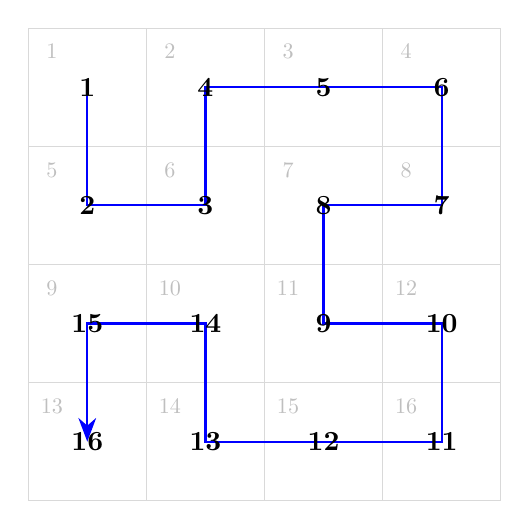
\begin{tikzpicture}[scale=1.5]
    % Draw the grid
    \draw[step=1cm, gray!30, thin] (0,0) grid (4,4);

    % Original pixel labeling (left-to-right, top-to-bottom)
    % Convention: (column, row) mapping to 1D index
    \foreach \y [evaluate=\y as \rowindex using int(4-\y)] in {1,2,3,4}
        \foreach \x [evaluate=\x as \colindex using int(\x-1)] in {1,2,3,4}
            \node[gray!50, scale=0.8] at (\x-0.8, \y-0.2) {\the\numexpr \rowindex*4 + \colindex\relax};

    % The Gilbert/Hilbert Path Coordinates for 4x4
    % Sequence: (0,0), (0,1), (1,1), (1,0), (2,0), (3,0), (3,1), (2,1), (2,2), (3,2), (3,3), (2,3), (1,3), (1,2), (0,2), (0,3)
    % Adjusted to grid centers (0.5 offset) and flipped Y for top-down
    \draw[thick, blue, -{Stealth[length=3mm]}] 
        (0.5, 3.5) -- (0.5, 2.5) -- (1.5, 2.5) -- (1.5, 3.5) -- 
        (2.5, 3.5) -- (3.5, 3.5) -- (3.5, 2.5) -- (2.5, 2.5) -- 
        (2.5, 1.5) -- (3.5, 1.5) -- (3.5, 0.5) -- (2.5, 0.5) -- 
        (1.5, 0.5) -- (1.5, 1.5) -- (0.5, 1.5) -- (0.5, 0.5);

    % Relabeling g(1)...g(16)
    \coordinate (P1)  at (0.5, 3.5); \node[font=\bfseries] at (P1) {1};
    \coordinate (P2)  at (0.5, 2.5); \node[font=\bfseries] at (P2) {2};
    \coordinate (P3)  at (1.5, 2.5); \node[font=\bfseries] at (P3) {3};
    \coordinate (P4)  at (1.5, 3.5); \node[font=\bfseries] at (P4) {4};
    \coordinate (P5)  at (2.5, 3.5); \node[font=\bfseries] at (P5) {5};
    \coordinate (P6)  at (3.5, 3.5); \node[font=\bfseries] at (P6) {6};
    \coordinate (P7)  at (3.5, 2.5); \node[font=\bfseries] at (P7) {7};
    \coordinate (P8)  at (2.5, 2.5); \node[font=\bfseries] at (P8) {8};
    \coordinate (P9)  at (2.5, 1.5); \node[font=\bfseries] at (P9) {9};
    \coordinate (P10) at (3.5, 1.5); \node[font=\bfseries] at (P10) {10};
    \coordinate (P11) at (3.5, 0.5); \node[font=\bfseries] at (P11) {11};
    \coordinate (P12) at (2.5, 0.5); \node[font=\bfseries] at (P12) {12};
    \coordinate (P13) at (1.5, 0.5); \node[font=\bfseries] at (P13) {13};
    \coordinate (P14) at (1.5, 1.5); \node[font=\bfseries] at (P14) {14};
    \coordinate (P15) at (0.5, 1.5); \node[font=\bfseries] at (P15) {15};
    \coordinate (P16) at (0.5, 0.5); \node[font=\bfseries] at (P16) {16};
\end{tikzpicture}
\caption{$4 \times 4$ 矩形上的一个 Gilbert 曲线示例。灰色数字表示原始索引，黑色数字表示重排后的索引。换言之，$g(\text{黑色}) = \text{灰色}$。注意此处的 Gilbert 曲线与 \texttt{gilbert\_curve.cpp} 中实际实现的 Gilbert 曲线略有不同。}
\label{fig:gilbert_curve}
\end{figure}

如果朴素地计算 Gilbert 曲线，人们可能会想到：将 $w \times h$ 矩形“填充”到包含它的最小 $2^n \times 2^n$ 正方形，在该正方形上计算 Hilbert 曲线，然后截去矩形之外的曲线部分。然而这样计算效率较低，因为通常会有超过一半的计算资源浪费在矩形外区域。这里我们采用两种更高级的方法。

\subsubsection{紧凑 Gilbert 曲线（Compact Gilbert curves）}

该方法\footnote{参见 ``Compact Hilbert indices: Space-filling curves for domains with unequal side lengths.'' 可见 \url{https://doi.org/10.1016/j.ipl.2007.08.034}.} 由 Chris H. Hamilton 和 Andrew Rau-Chaplin 提出，先计算
\begin{equation}
    w^* = \lceil \log_2(w) \rceil, \qquad h^* = \lceil \log_2(h) \rceil
\end{equation}
它们分别是表示一个 $x$ 索引与 $y$ 索引所需的比特数（$0$ 或 $1$）。该方法对给定点 $(x,y)$，从最粗（最高）比特层开始，判断该点在当前比特层所处象限并设置对应比特，然后进入下一层（更低层），重复此过程。

在过程结束时，可以得到一个索引 $0 \leq C(x, y) \leq 2^{w^* + h^*} - 1$，它描述了该点在 Gilbert 曲线上的位置。对所有 $0 \leq x < w$ 与 $0 \leq y < h$ 计算 $C(x,y)$ 后，得到\emph{未归一化}紧凑 Gilbert 函数
\begin{equation}
    C\colon \{0, 1, \ldots, w h - 1\} \to \{0, 1, \ldots, 2^{w^* + h^*} - 1\}.
\end{equation}
该映射是单射，但通常不是满射。我们通过对输出值排序并取秩来归一化 $C$，得到\emph{归一化}紧凑 Gilbert 函数
\begin{equation}
    \tilde{g}\colon N = \{0, 1, \ldots, w h - 1\} \to N, i \mapsto \text{$C(i)$ 在 $C(N)$ 中的秩}.
\end{equation}
这个 $\tilde{g}$ 满足：$\tilde{g}(i)$ 是索引为 $i$ 的点在“截断曲线”上的位置。对 $\tilde{g}$ 取逆可得
\begin{equation}
    g\colon \{0, 1, \ldots, w h - 1\} \to \{0, 1, \ldots, w h - 1\}, i \mapsto \tilde{g}^{-1}(i)
\end{equation}
它给出了曲线上第 $i$ 个点对应的像素索引。这个 $g$ 就是我们所需的置换 $\sigma$。

\subsubsection{精确 Gilbert 曲线（Exact Gilbert curves）}

该方法\footnote{参见 \url{https://github.com/jakubcerveny/gilbert/}.} 由 Jakub Červený 提出，通过递归地将矩形沿 U 形路径分成三个区域，构造一条完全在 $w \times h$ 矩形内部行进的曲线。注意在某些特殊情况下会使用对角移动。该方法给出一个\emph{归一化}精确 Gilbert 函数
\begin{equation}
    g\colon \{0, 1, \ldots, w h - 1\} \to \{0, 1, \ldots, w h - 1\}
\end{equation}
它给出了曲线上第 $i$ 个点对应的像素索引。

参考常用工具“小番茄图片混淆”\footnote{参见 \url{https://xfqtphx.netlify.app/}.}，在这一情形下我们并不直接将此 $g$ 用作置换。相反，我们沿精确 Gilbert 曲线将每个像素整体平移一个偏移量
\begin{equation}
    k = \Bigl\lfloor \frac{\sqrt{5} - 1}{2} h w \Bigr\rceil = \Bigl\lfloor \frac{h w}{\varphi} \Bigr\rceil.
\end{equation}
这意味着：新图像中索引为 $j$ 的像素（它原本是曲线上第 $g^{-1}(j)$ 个点）在平移后应当来自曲线上第 $(g^{-1}(j) - k)$ 个点。由于 $g$ 为双射，存在某个 $i$ 使得 $j = g(i)$。因此我们所需的置换为
\begin{equation}
    \sigma\colon \{0, 1, \ldots, w h - 1\} \to \{0, 1, \ldots, w h - 1\}, g(i) \mapsto g(\overline{i - k})
\end{equation}
其中 $\overline{i - k}$ 按 $\bmod \; h w$ 理解。注意由于 $g$ 是双射，该置换是良定义的。

\subsection{混沌系统}

如果我们只想得到一个高度“噪声化”但可复现的 $\sigma$（例如 Cloudflare 旧金山办公室的熔岩灯能够产生非常嘈杂的数据，但之后几乎不可能反求出置换），那么可以考虑混沌系统。非常宽松地说\footnote{严格地讲，混沌系统有多种严谨数学定义。最经典的一种是定义在度量空间 $(X,d)$ 上连续函数 $f\colon X \to X$ 的 Devaney 混沌：若 $f$ 拓扑传递、周期点稠密，并且对初值敏感，则称其为 Devaney 混沌。不过这里我们把这些内容留到数学课中讨论。}，我们用以下性质来刻画混沌系统：
\begin{itemize}
    \item 系统以确定性方式演化。也就是说，总存在明确函数 $f$，使得 $x_{n + 1} = f(x_n)$。
    \item 对任意初始状态，只要时间足够长，系统都可以演化到任意区域。
    \item 系统对初始条件敏感。即两个非常接近的初始点，之后可能演化出截然不同的轨迹。
\end{itemize}

有许多简单函数 $f\colon I \subseteq \mathbb{R} \to \mathbb{R}$ 会表现出混沌行为。例如，当 $r \lesssim 4$ 时的 logistic 映射 $L(x) = r x (1 - x)$，参数 $\mu \in (1, 2)$ 时的 tent 映射 $T(x) = \mu \min\{x, 1 - x\}$（见图~\ref{fig:tent_map}），以及倍增映射 $D(x) = 2 x \pmod 1$，都可用于模拟混沌。

\begin{figure}[b!]
    \centering
    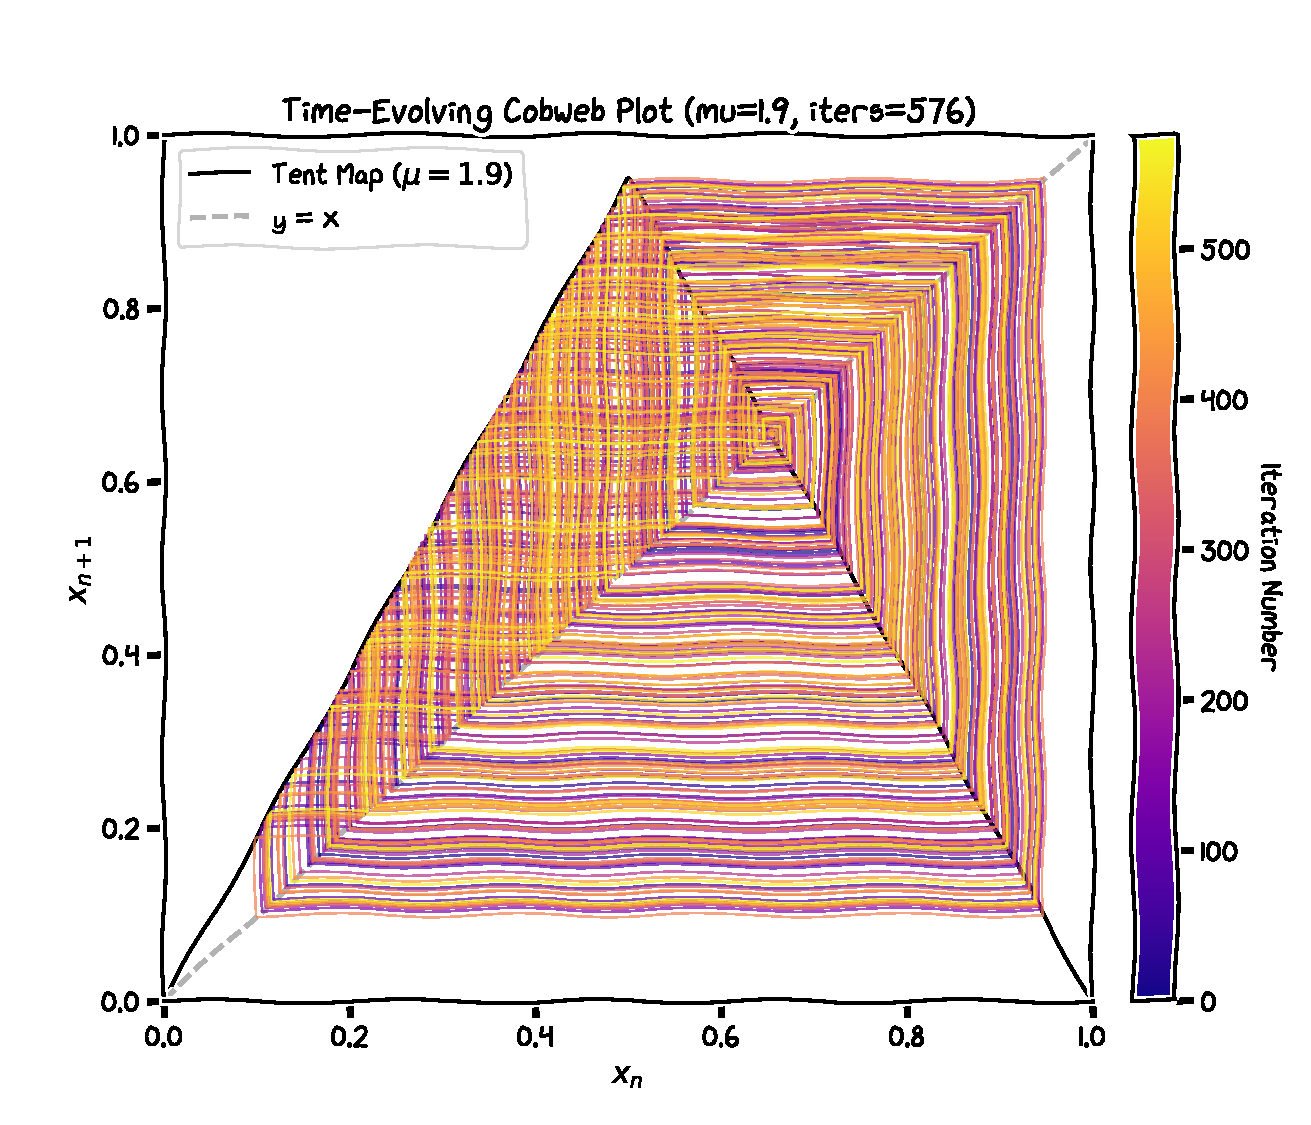
\includegraphics[width=0.6\linewidth]{figures/tent_map.pdf}
    \caption{取 $\mu = 1.9$、$x_0 = 0.7$ 时，tent 映射迭代 ${24}^2$ 次后的演化。}
    \label{fig:tent_map}
\end{figure}

设一个混沌映射 $f\colon I \subseteq \mathbb{R} \to \mathbb{R}$。用户定义的种子 $s$ 给定初始条件 $x_0 = s$。对 $0 \leq i < w h - 1$，计算
\begin{equation}
    x_{i + 1} = f(x_i).
\end{equation}
这将得到一个类似噪声的数组 $(x_n)_n$。我们可通过排序对 $x_n$ 取秩，并在必要时使用下标 $n$ 打破并列，从而得到所需置换
\begin{equation}
    \sigma\colon \{0, 1, \ldots, w h - 1\} \to \{0, 1, \ldots, w h - 1\}, i \mapsto \text{使得 $x_n$ 的秩为 $i$ 的那个 $n$}.
\end{equation}

\subsubsection{Tent 映射}

我们实现的 tent 映射为
\begin{equation}
    T_\mu\colon [0, 1] \to [0, 1], x \mapsto 
    \begin{cases}
        \mu x & x < 1/2, \\
        \mu (1 - x) & x \geq 1/2
    \end{cases}
\end{equation}
其中 $0 < \mu \leq 2$。该映射在 $\mu = 2$ 时具有很强的混沌性。然而在实际 C++ 实现中，乘以 $2$ 基本等价于按位左移。由于精度有限，大约迭代 53 次后所有有效比特都会丢失。因此我们取 $\mu = 1.9999$。

\pagebreak

\appendix

\section*{附录}

\setcounter{figure}{0}
\renewcommand{\thefigure}{A\arabic{figure}}

\setcounter{table}{0}
\renewcommand{\thetable}{A\arabic{table}}

\section{permutations 模块的头文件}

\lstinputlisting[language=C++]{../permutation.h}

\clearpage

\section{Gilbert 曲线模块的头文件}

\lstinputlisting[language=C++]{../gilbert_curve.h}

\clearpage

\section{混沌系统模块的头文件}

\lstinputlisting[language=C++]{../chaos.h}

\end{document}
